%
% Chapter 2
%

\chapter{EXPERIMENTS AND DATA ACQUISITION}

\section{Lifetime Measurements of Excited States}\label{sec:lifetime_measurement_techniques}
The measurement of excited state lifetimes remains an integral part in discerning information about the structure of the nucleus. An abundance of techniques, applicable/sensitive lifetime ranges, and facilities can be implemented to measure these lifetimes in the massive landscape of existing isotopes in nuclei. A schamatic of experimental measures available for use with several lifetime measurement techniques can be found in Figure \ref{fig:VariousLifetimeMeasurements}:

\begin{figure}[h!] 
\begin{center}
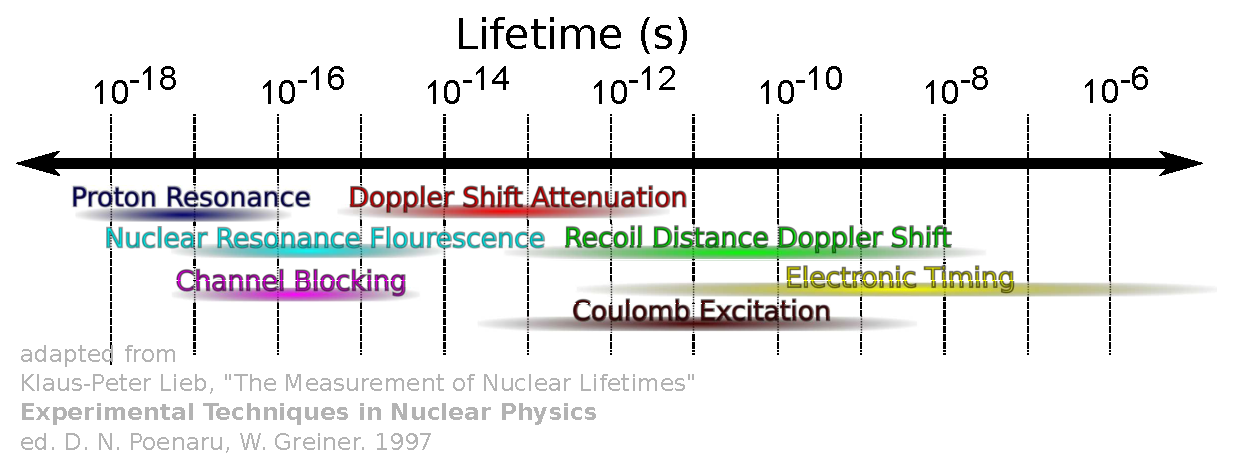
\includegraphics[width=0.95\textwidth]{figures/lifetimes-techniques-full.eps}
\caption{Techniques available to nuclear physicists to measure lifetimes as short as a few attoseconds (10$^{-18}$~s) to the more long-lived lifetimes on the order of microseconds (10$^{-6}$~s) (Adapted from \cite{Poenaru_text}, courtesy of M.~K. Smith).}
\label{fig:VariousLifetimeMeasurements}
\end{center}
\end{figure}

The various lifetime measurement techniques span a tremendous and continuous range of possible lifetimes for nuclear excitations, from $\sim$10$^{-18}$ to $\sim$10$^{-6}$~s, and can be applied to the vast majority of the $\sim$3339 known nuclei in existence (stable and unstable). Several lifetime measurement techniques directly measure the lifetime (or a lifetime-dependent factor in the case of the Doppler Shift Attenuation Method) via various means; techniques like the Recoil Distance Doppler Shift, Coulomb Excitation, and Electronic Timing rely on fast-timing techniques for multiple $\gamma$-ray and/or particle coincidences to measure the lifetimes of metastable states. These direct lifetime measurements apply to the longer-lived excitations (picosecond and above lifetimes), and are contrasted with the more exotic, indirect methods (Proton Resonance, Nuclear Resonance Flourescence, and Channel Blocking) that measure the partial or total Lorentzian energy ($\Gamma\approx\hbar$/$\tau$) width(s) to extract the lifetime of a state. Each lifetime measurements also has its own set of experimental advantages and challenges in addition to their respective sensitive ranges of lifetime measurement. For example, Electronic Timing can measure lifetimes over a very broad range of lifetimes by measuring the time between successive decays into and out of a state, but is limited by the requirement that the particular state desired must be populated via a cascade from higher-lying levels or by charged particle decays. Coulomb excitation offers a relatively simple measurement technique, in that it can directly deduce nuclear lifetimes by measuring the reduced transition probability for direct population of a desired state from the ground state, however, for decays that are not directly linked to the ground state via $\gamma$ decay, this method rapidly increases in complexity. The Recoil Distance Doppler shift method utilizes Doppler-type effects to measure intensities of decay radiation as a function of target position (which then correlates to a nuclear lifetime). This picosecond-range lifetime measurement technique is highly tunable to the precise needs of the experimentalist, yet the methodology and necessary experimental equipment needed can become cumbersome and sophisticated.

Specifically, level lifetimes in the tens to hundreds of femtosecond ($\sim$10$^{-15}$ s) range can be measured with the Doppler Shift Attenuation Method (DSAM), a technique that exploits a recoiling nucleus to produce Doppler shifted $\gamma$-rays when observed at various laboratory angles. The magnitude of the Doppler shift is reliant on a lifetime-dependent factor, which we can easily extract from experiments in the laboratory. DSAM holds a unique place in the overall landscape of lifetime measurement techniques in that it is almost exclusively sensitive in this near-femtosecond timescale. The level lifetimes from DSAM can then be quickly extracted from the angular energy shift(s) of any $\gamma$-rays that de-excite the nucleus.  All of the presented lifetimes in this work are measured with this DSAM technique at the University of Kentucky.

\section{DSAM-INS Formalism}
A $\gamma$-ray observed from a recoiling nucleus will be energy-shifted linearly as a function of the laboratory angle, \textit{$\theta_{lab}$}, shown in Equation \ref{eq:F(tau)}. This angular dependence on the energy is due to observation of Doppler shifted energies of the $\gamma$-ray, based on the detection angle, $\theta_{lab}$, as a $\gamma$ ray observed as the nucleus recoils `away' from the observer will be `red-shifted' down in energy, and inversely (energies will be `blue-shifted') for a $\gamma$ ray observed for nuclei that recoil `towards' the detector.

\begin{equation} \label{eq:F(tau)}
E_{\gamma}(\theta_{lab})=E_{\gamma,o}[1+\beta F(\tau) \cos(\theta_{lab})]
\end{equation}

Here, \textit{E$_{\gamma,o}$} is the unshifted $\gamma$-ray energy, \textit{F}(\textit{$\tau$}) is an attenuation factor, dependent on the lifetime of the excited state (to be discussed in detail in \S \ref{sec:AD_Ft}, as this is one of the key experimental quantities we measure), and $\beta$ is the ratio of the recoil velocity of the target nucleus to the speed of light, \textit{c}; this recoil velocity is derived in Pelte and Schwalm \cite{Pelte_text} from the kinematics involving conservation of momentum and energy in the laboratory frame, and is given by Equation \ref{eq:betarecoil}. 

\begin{equation} \label{eq:betarecoil}
\beta=0.04635 \frac{A_n}{A_n+A_A}\sqrt{\frac{E_n}{A_n}}
\end{equation}

The mass numbers of the bombarding particle and solid target are \textit{A$_n$} and \textit{A$_A$}, respectively, with the bombarding particle energy given by E$_n$ in MeV. In (n,n$^{\prime}\gamma$) experiments, \textit{A$_n$} is unity, while \textit{A$_A$} must take into account the full molecular weight of the target, \textit{e.g.} for Dysprosium-Oxide powder ($^{162}$Dy$_2^{16}$O$_3$), \textit{A$_A$}=162$\times$2+16$\times$3=372. For rare-earth nuclei and \textit{E$_n$}$<$5~MeV, the nuclear recoil velocities are generally less than 1~\% of the speed of light, meaning relativistic effects do not need to be taken into account as they normally would with other lifetime measurement techniques (\textit{e.g.} Recoil Distance Doppler Shift measurements). For example, the recoil velocity $\beta$ for a $^{162}$Dy$_2^{16}$O$_3$ molecule recoiling from a bombarding neutron of 3.1~MeV is 2.1878e-~4. Lifetimes, then, are measured via the single experimental observable, the energy of the $\gamma$ ray as a function of angle; this is achieved at the University of Kentucky with High Purity Germanium detectors with high-resolution $\gamma$-ray spectroscopy to measure precise energy shifts. This excellent energy resolution provided by HPGe detector systems is ideal to measure the $\sim$200-300~eV energy shifts needed, as older fast NaI(Tl) detectors cannot distinguish peaks at such a fine-grain resolution. To highlight this centroid energy shift, Figure \ref{fig:spectra_shift_DSAM} shows a 1902.055~keV $\gamma$-ray Doppler shifting as the detector changes laboratory angle, with the centroids drawn to guide the eye.

\begin{figure}[h] 
\begin{center}
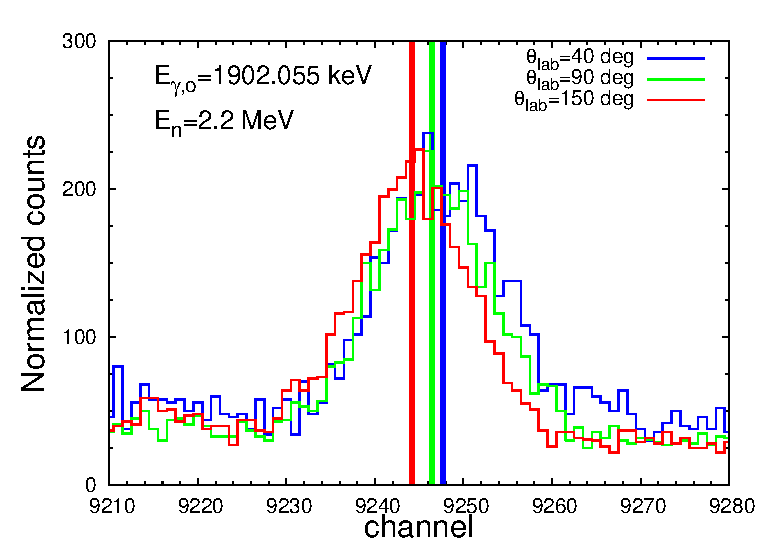
\includegraphics[width=0.97\textwidth]{figures/spectra_shift_DSAM.eps}
\caption{Doppler shift of an E$_\gamma$=1902.055~keV de-excitation from the $\theta_{lab}$=40, 90, and 150 degrees in red, blue, and green, respectively. The vertical lines mark the centroid of each peak of corresponding color.}
\label{fig:spectra_shift_DSAM}
\end{center}
\end{figure}


From Equation \ref{eq:F(tau)}, the only undetermined parameter is \textit{F}(\textit{$\tau$}), an attenuation factor directly dependent on the specific lifetime of the decaying state, formulated by Blaugrund in ref. \cite{BLAUGRUND_DSAM_1966} to be an effect of the recoil nuclei slowing down in the target medium while they decay. \textit{F}(\textit{$\tau$}) can be calculated via multiple formulations, where all formulations rely on an understanding of the nuclear and electronic stopping power of a medium to produce this lifetime dependent attenuation, as the inelastic interaction of the bombarding particle is directly related to these stopping powers. In this work, the Winterbon formalism will be used, where the underlying framework is outlined in \cite{WINTERBON_1975} and \cite{Belgya_DSAM1996}, where an exact solution was obtained for the attenuation factor \textit{F}(\textit{$\tau$}) in terms of the electronic stopping power, the nuclear scattering cross sections, and target density. Key improvements were made to this attenuation factor calculation in the early 1970s by taking the possibility of nuclear deflection during the recoil as well as slowing inside the material lattice into account. This refinement is a necessary addition with the use of large, molar amounts and physical weights of target material, where the electronic stopping power of the medium plays a finite aspect in the calculation of the Winterbon curve; previous (Lindhard and Blaugrand) formulations of the theoretical \textit{F}(\textit{$\tau$}) factors were unable to successfully represent both the nuclear and electronic stopping powers correctly, vastly and systematically underestimating the attenuation. Further advancement of the Winterbon formalism was investigated in \cite{PETERS_DSAM2013}, with attention being placed on the chemical makeup of the target to better characterize the lattice relaxation needed to quantify the nuclear recoil inside the sample. This placed an important focus on the dependence on the oxide powder's consistency and packing density of the molar quantity of the target material inside a container (in our case, a polyethelene vial) when calculating the Winterbon curve.
% [NEED LARGE AMOUNT OF MATERIAL TO PROVIDE STOPPING POWERS (LATTICE NEEDS TO RELAX)]

Note that energy shifts (and thus F($\tau$)) must \textit{always} be positive, in that energies of DSAM $\gamma$ rays are higher at forward angles and lower at backward angles for any realistic system. We will encounter some of the limitations behind measurement of $\gamma$ ray energies via DSAM shortly, and oftentimes, the measured energy shift is either consistent with zero or negative. These limitations in an extraction of F($\tau$) are products of either a lifetime that is outside the range of DSAM, or other factors including sample self-attenuation and/or coincidence with background radiation to blur the centroid energy shift of a particular $\gamma$ ray.

\section{(n,n$^{\prime}\gamma$) Experiments at the University of Kentucky}
DSAM requires the nucleus to be moving as it decays from an excited state for it to be effective, and the preferred probe to excite the nucleus used at the University of Kentucky Accelerator Laboraty (UKAL) is the inelastic scattering of neutrons. The inelastic scattering reaction imparts some velocity to the target nuclei, fulfilling the base requisite for DSAM, that the target is moving as it decays. In years past, thermal neutrons from various fission sources have been utilized to perform the inelastic scattering reactions, but the accessibility of monoenergetic neutrons has made UKAL a popular and unique setting in the realm of experimental structure physics. Energetic neutrons cannot be accelerated with a standard electrostatic accelerator due to their neutral charge-state, so non-thermalized neutrons must be produced via a primary reaction. This mechanism is outlined in Equation \ref{eq:3HQvalue}.
\begin{equation} \label{eq:3HQvalue}
\text{${}^3$H(p,n)${}^3$He, Q = -0.763 MeV}
\end{equation}

This $^3$H(p,n) reaction produces quasi-monoenergetic neutrons, tunable to a desired energy in a 0.5~-~5.5~MeV bombarding neutron energy range, ideal for studying the low-lying states in nuclei. UKAL uses their on-site 7~MV single-ended Van DeGraff accelerator to accelerate a bunched, pulsed beam (at a frequency of 1.875~MHz) of protons to impinge on a pressurized (slightly above atmospheric at $\sim$110 kPa) tritium gas cell, prompting the reaction to produce a forward cone of neutrons. A slight energy spread is present in the outgoing neutrons due to a thin molybdenum foil to prevent the gas cell from out-gassing upstream, which would catastropically contaminate the entire beamline with radioactive $^3$H. This energy straggling is minute, however, providing a $\sim$2.5\% energy spread on average at 50-100~keV standard deviation on neutron energy \cite{Belgya_DSAM1996}. %A forward-monitor measurement of this neutron energy spread is shown in [FIGURE HERE AND ASK SHELLY ABOUT FWD MONITOR] and is typically on the order of $\sim$50~keV. 

The choice of neutrons as a probe can be justified for multiple reasons, and brings its set of distinct advantages; the inelastic scattering and low-spin transfer leaves the nucleus in excited, aligned states with relatively low angular momentum. Generally, spin 5$^{\pm}$ states are the practical limit of angular momentum that can be imparted in an inelastic scattering reaction with neutrons at the University of Kentucky. This low-spin population of states is because the spin-1/2 neutron would naturally not be able to produce a higher spin state without the addition of a very large amount of angular momentum during the inelastic scattering reaction. The neutral charge of the neutron also implies that the scattering reaction is not impeded by the Coulomb barrier; this means that levels are populated very close to the bombarding neutron energy. Lastly, the excited states populated by inelastic neutron scattering are generally nonselective, in that either single-particle excitations or collective states can be populated, allowing the study of both types of excitation. The Doppler Shift method also offers the unique ability to tune bombarding neutron energies to populate states at or very near their threshold energies. This effect is two-fold: first, the experimentally determined F($\tau$) factor from Equation \ref{eq:F(tau)} is directly dependent on the incoming neutron energy, so minimization of the neutron energy is key to extraction of the lifetime, so the `observed' F($\tau$) will be inflated for higher neutron energies. Secondly, this `dialing-in' of neutron energy can completely remove any lifetime inflation due to feeding from higher-lying states; DSAM is unique in this aspect because the other methods of measuring a nuclear lifetime will be unable to remove this feeding, or in some cases (such as the Gamma Ray Induced Doppler Broadening technique), the feeding will manifest as a large uncertainty in measurement.

DSAM following inelastic neutron scattering is not without its downsides or experimental challenges to overcome. Since the target has significant thickness and involves molar quantities of target powder, $\gamma$ rays from deep inside the sample will be attenuated in their trajectory out of the sample. This has a two-fold effect, in that the absolute intensity must be corrected for (explained in detail in \S \ref{sec:gambit_correction}) low-energy $\gamma$ rays that could easily become fully attenuated and absorbed by the target material, and that any lifetimes extracted from the linear shift of energy \textit{may} not be trustworthy, as the energy attenuation is strongly angular dependent, effectively `flattening' the Doppler energy shift. 

The ensemble of (n,n$^\prime\gamma$) experiments performed at UKAL can be achieved with the relatively simple experimental setup, shown in Figure \ref{fig:ExpSetup}.

\begin{figure}[h!] 
\begin{center}
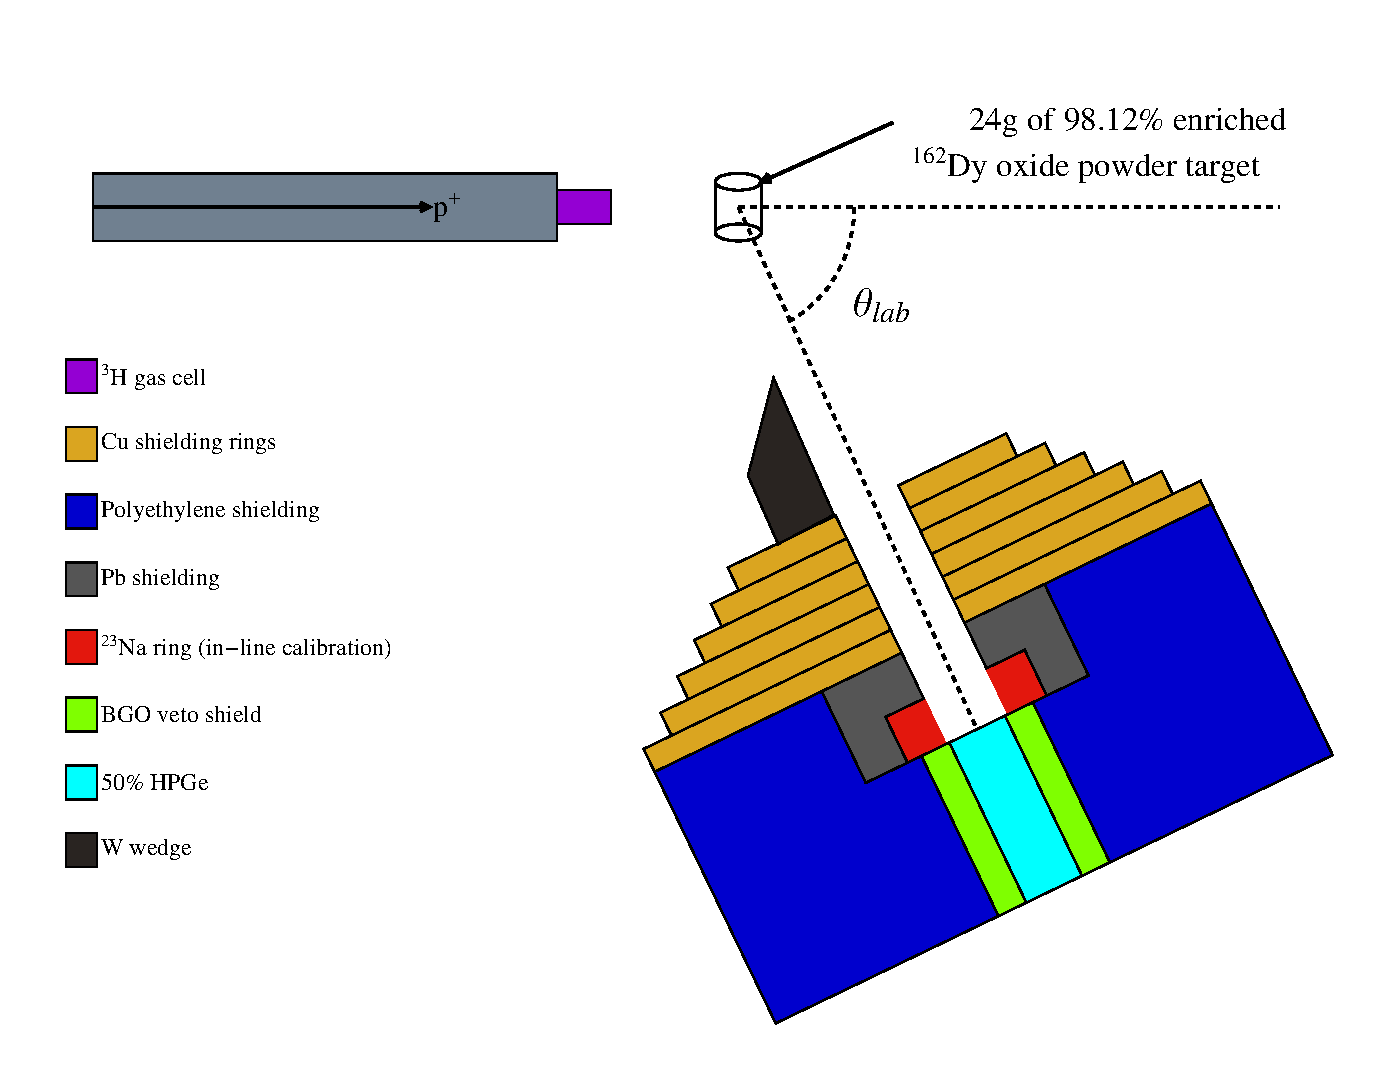
\includegraphics[width=0.97\textwidth]{figures/SciDraw_ExpSetup_Dy.eps}
\caption{Sample Experimental Setup at UKAL for $\gamma$-singles measurements (Made in M. Caprio's SciDraw software for Mathematica \cite{Caprio2005107})}
\label{fig:ExpSetup}
\end{center}
\end{figure}

The single 50\% relative efficiency Ortec HPGe planar detector (named after the 1904 Kentucky Derby winner Elwood) sits $\sim$125~cm away from the end of the beamline on a goniometer equipped circular track $\sim$2~m in radius to observe $\gamma$-rays at various laboratory angles. In Figure \ref{fig:ExpSetup}, the target (a cylindrical polyethelene vial of enriched target powder) is suspended a few ($\sim$4) inches away from the end of the tritium gas cell, where monoenergetic neutrons will inelastically scatter off the target, prompting $\gamma$ decay from the sample to be observed by the HPGe detector. The proximity of the target in relation to the end of the tritium gas cell ensures that the highest possible neutron flux from the forward cone of neutrons will strike the majority of the target material. The castle of passive shielding materials are two-fold in use: to lower background radiation in spectra and to diminish fast neutron damage to the HPGe detector itself. The viewing channel of the detector is lined with copper plating to absorb fast neutrons from the tritium gas cell at the end of the beamline. In addition, borated polyethelene surrounds the detector to reduce secondary \& tertiary scattering of neutrons and $\gamma$-rays from reaching the detector; the typical ensemble of lead rings also aid in regular $\gamma$ background reduction. Lastly, a wedge of tungsten is placed in direct view of the tritium gas cell to act as a shadow bar to prevent neutrons from directly entering the detector from the gas cell. An ensemble of BGO (Bismuth Germanate Oxide) scintillators are placed annularly around the HPGe detector to further aid in Compton scattering background suppression; these scintillation detectors provide an anti-coincidence to veto background events that occur, actively cleaning spectra.

Spectra are generated from the Time of Flight (TOF) technique to discriminate background events from prompt $\gamma$ events; a time-to-amplitude converter (TAC) measures the relative time between events in the HPGe detector and a beam pick-off signal near the end of the beamline. At UKAL, the events in the HPGe act as the `start' and the pick-off serves as the `stop' as to not flood the electronics from pick-off signals that do not result in detected radiation. The concept of the TOF technique is that particles and $\gamma$-rays require different amounts of time to reach a detector, dependent on their velocity (neutrons of a velocity $\ll$ \textit{c} take longer to reach a detector than a $\gamma$-ray traveling at the speed of light). This time difference between measured events is recorded by the TAC, and TOF spectra are generated through a built-in single channel analyzer (SCA). Specifically at UKAL though, the neutron events occur \textit{first} as they scatter off the various materials (mainly primary scattering off iron) in between the target and detector face, while the speed of light $\gamma$-ray events occur in the larger peak. The resultant spectrum is used to properly gate the experimental datasets in the analog-to-digital converter (ADC) by only selecting corresponding prompt $\gamma$-ray events from the histogram. An example of a typical TOF spectrum from experiments at UKAL is shown in Figure \ref{fig:TOF_spec}.

\begin{figure}[h] 
\begin{center}
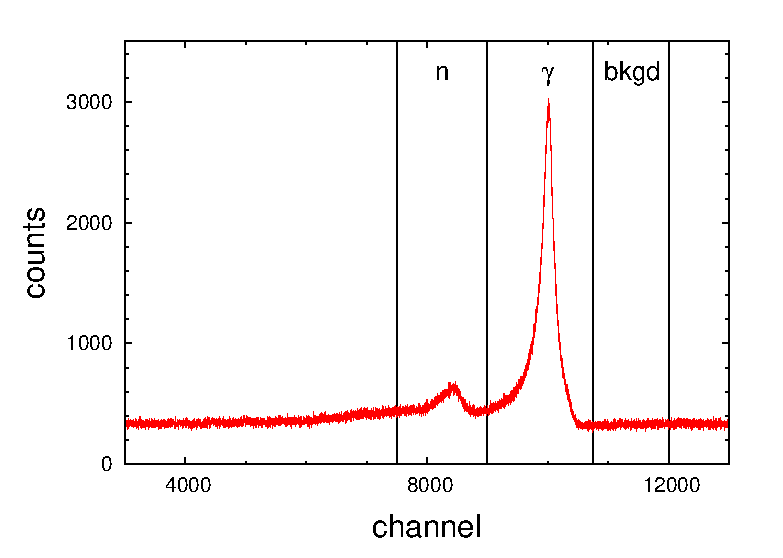
\includegraphics[width=0.97\textwidth]{figures/TAC_spectrum.eps}
\caption{Typical TOF spectrum with labeled regions for corresponding $\gamma$, neutron, and background events.\label{fig:TOF_spec}} %Note the passage of time to the left, starting at the prompt $\gamma$-ray peak, followed by a neutron bump, and wrapping back around the x-axis.
\end{center}
\end{figure}

The single-detector setup and $\gamma$-singles based experiments provide more distinct downsides to lifetime measurements via DSAM at the University of Kentucky in particular. The limitations of not using $\gamma$-$\gamma$ coincidences can have profound implications on the visibility and overall statistics of spectra gathered from the experiment(s); being able to apply timing gates on individual $\gamma$-decays is an extremely powerful tool in determining decay patterns, cascades, and lower-intensity peaks for interband decays. One detector setups require a considerable length to the experimental campaign, and is a severe limitation to the facilities, where the experimenters must enter the target room periodically throughout the run to physically move the detector across the entire range of angles used in the measurements, and must systematically scan through the entire range one angle at a time. Given an unlimited amount of beamtime with little to no deadlines, this is not a problem, however, a modest amount of statistics for $\gamma$-decays observed in a typical measurement require up to (in some cases in excess) a week of continuous beamtime for a single neutron energy angular distribution. 
% Background-subtracted spectra are then generated by subtracting any events that correspond to the random background region from the prompt $\gamma$-ray gated events from the TAC spectrum in Figure \ref{fig:TOF_spec}.

\subsection{Excitation Function Measurements}
Typically, the first measurements to be made are excitation function measurements; these supplement the $\gamma$-singles nature of the angular distribution measurements, to help infer the ideal bombarding neutron energy for peak $\gamma$-ray population rates. In stark contrast to the angular distributions where the neutron energy is kept constant, the excitation functions modulate the bombarding neutron energy to provide the $\gamma$-ray population strengths as a function of neutron energy. Similarly in contrast, the HPGe detector is kept at a constant laboratory angle of 90 degrees with respect to the beamline. An extremely powerful tool, these excitation functions provide important insight into the nature of any observed $\gamma$-rays; for a particular excited state that de-excites via multiple channels, the corresponding $\gamma$-rays will have both the same a) quantitative threshold, and b) qualitative shape. The absolute threshold allows previously unidentified or unplaced $\gamma$-ray transitions to be placed into a known level scheme, as the threshold for the de-excitation must match the level energy. If the populated level's spin are high (5$^\pm$), the threshold will be higher than the level energy, as the bombarding neutron must have higher linear momentum (energy) to successfully provide enough angular momentum transfer during the reaction. The qualitative shape of the excitation functions is heavily dependent on the initial spin and parity of the de-exciting level, making $\gamma$-ray discrimination and identification from different levels a trivial task. This identical shape also allows the relative intensities of $\gamma$-rays to be inferred (independent of the absolute intensities we can gather from the angular distribution measurements), since we can take the ratio of matched-shape excitation functions. An example of two matching $\gamma$-ray transitions from the same level (J$^\pi$=5$^-$), contrasted with a $\gamma$-ray from another level (J$^\pi$=1$^-$) is shown in Figure \ref{fig:matching_exf}. 

\begin{figure}[h] 
\begin{center}
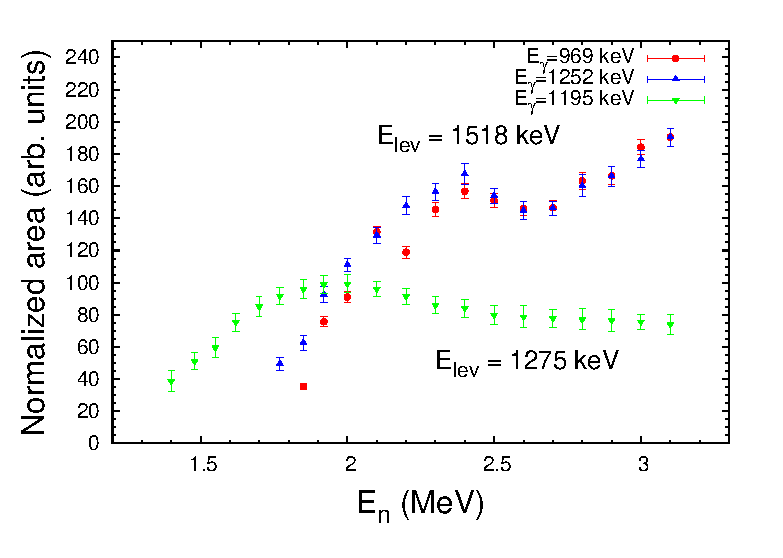
\includegraphics[width=0.97\textwidth]{figures/matching_exf.eps}
\caption{Superimposed excitation functions for two gamma rays (E$_\gamma$=969 \& 1252~keV) leaving the same level (E$_{lev}$=1518~keV), and a single 1195~keV $\gamma$-ray leaving a separate E$_{lev}$=1275~keV level in $^{162}$Dy. The different thresholds and shape of the 1195~keV and 969~keV de-excitations imply that these decays are from two different levels, clearly showing their placement in the level scheme.}
\label{fig:matching_exf}
\end{center}
\end{figure}

The excitation function measurements serve as a quasi-replacement for $\gamma$-$\gamma$ coincidences in a particular experiment, as it allows retention of good statistics that one would get from $\gamma$-singles spectroscopy. With $\gamma$-$\gamma$ coincidences, a level scheme can be built extremely easily, because coincident $\gamma$-decay chains into and out of levels are unquestionably vivid in multiple HPGe detectors; this is not the case in a $\gamma$-singles experiment, since a) particular $\gamma$-rays appear only in the single HPGe detector, and b) discrimination of decay chains is impossible with $\gamma$-singles. The excitation function allows a level scheme to be built in a similar fashion to $\gamma$-$\gamma$ coincidences, while only requiring a single detector, because threshold energies are obvious, and that the qualitative shape of the excitation functions will be identical. Without either implemented technique (excitation function measurements or $\gamma$-$\gamma$ coincidences), proper $\gamma$-spectroscopy would be rendered impossible, as we would no longer be able to confidently place $\gamma$ decays to levels or assign level lifetimes from the Doppler Shift Attenuation measurements.
%[EXPAND ON THIS, CAN BUILD LEVEL SCHEME IN SIMILAR WAYS, ETC].
\subsection{Angular Distribution Measurements}
To extract the lifetimes of excited states, the angular distribution of gamma rays must be measured, specifically, the energy dependence of $\gamma$ rays as a function of lab angle; this is achieved at UKAL with the same single High-Purity Germanium detector used in the excitation function measurements. By physically moving the HPGe detector to different laboratory angles on the circular track, we can extract multiple observable quantities from the angular distribution measurements. First, \textit{F}(\textit{$\tau$}) is found by plotting \textit{E$_{\gamma}$} as a function of cos($\theta$); the relation in Equation \ref{eq:F(tau)} states that the centroid energy shift of a $\gamma$-ray will be linear with cosine, with \textit{F}(\textit{$\tau$}) being the slope. Comparison of this experimental \textit{F}(\textit{$\tau$}) factor with the theoretical calculation for \textit{F}(\textit{$\tau$}) allows extraction of a lifetime \textit{$\tau$} for the decay radiation and excited state. Special care must be taken when measuring the lifetimes, because higher-lying levels can introduce feeding transitions into lower-lying states, inflating the measured lifetimes. Since the theoretical \textit{F}(\textit{$\tau$}) factor is directly dependent on the recoil velocity (the bombarding neutron energy), additional inflation will also be introduced when extracting lifetimes for levels far below the bombarding neutron energy. Performing the excitation function measurements first allows for the minimization of lifetime inflation while maximizing population rate for a particular excited state, as we know the approximate population as a function of bombarding neutron energy.   

When the nucleus decays from an aligned state, the classical radiation pattern of the $\gamma$-ray can be expressed by the sum of even Legendre polynomials as a function of $\cos(\theta)$ (Equation \ref{eq:angdistW}), where the coefficients for each order polynomial are directly related to the multipolarity of the transition. Realistically, only the coefficients a$_2$ and a$_4$ are considered, since the higher order terms correspond to the contributions from the insignificantly intense multipolarities for $\Delta$J$>$2.
%SHOW DERIVATION FIGURE HERE

\begin{equation} \label{eq:angdistW}
W(\theta)=\sum_{\text{even k}}\alpha_k\text{P}_k\cos(\theta) \Rightarrow W(\theta) \approx \text{A}_0[1+\text{a}_2\text{P}_2\cos(\theta)+\text{a}_4\text{P}_4\cos(\theta)]
\end{equation}

The anisotropic nature of the $\gamma$ radiation produced arises from the fact that parity conserving nuclear reactions, \textit{e.g.} (n,n$^{\prime}\gamma$), and a defined beam direction, create a plane of interaction . Otherwise, the random orientation of nuclei in space would mean all multipolarities of $\gamma$ radiation  have isotropic angular distributions. By comparing the relative magnitude and sign of the a$_2$ and a$_4$ coefficients, limits can be placed on both the spin and parity of the de-exciting level, because dipole and quadrupole radiation patterns have distinct shapes (shown in Figure \ref{fig:multipole_diff}). These same Legendre Polynomial coefficients can also be compared to theoretical calculations to extract multipole mixing fractions ($\delta$) for mixed-multipolarity transitions. This multipole mixing fraction is simply the ratio of E2 transition strength to M1 transition strength:

\begin{equation} \label{eq:multipolemixing}
\delta=\frac{\langle\eta\vert E2 \vert\nu\rangle}{\langle\eta\vert M1 \vert\nu\rangle}
\end{equation}

\begin{figure}[h] 
\begin{center}
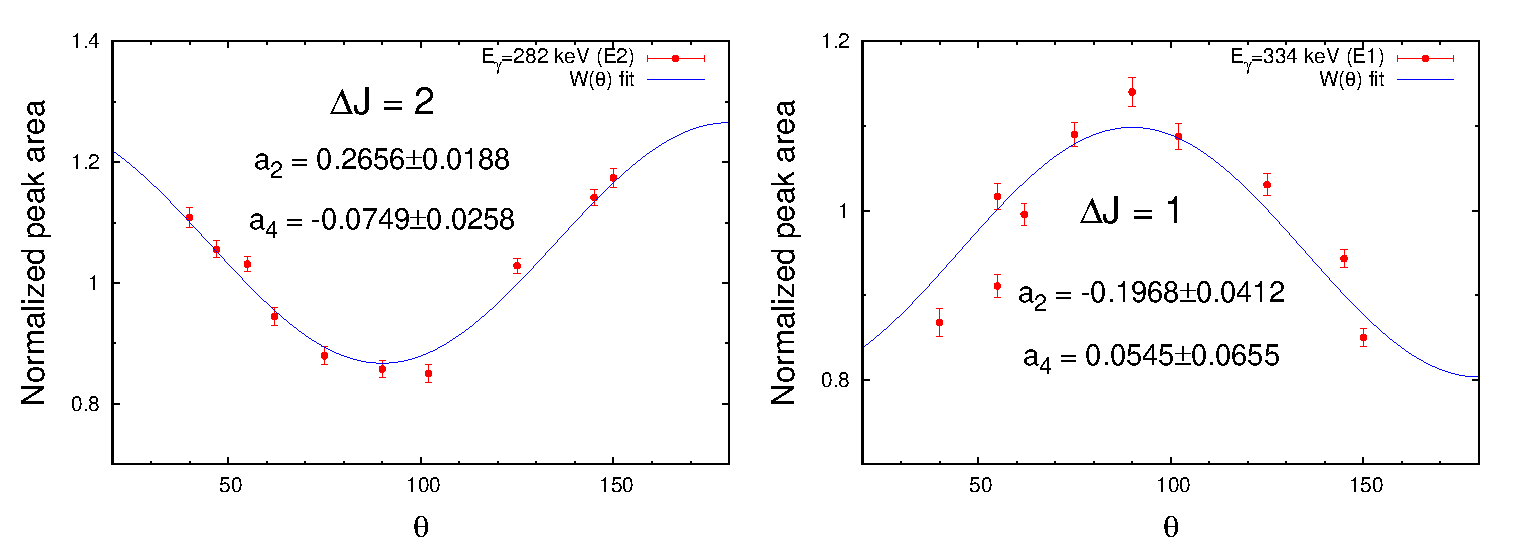
\includegraphics[width=0.97\textwidth]{figures/multipole_diff.eps}
\caption{Angular distributions for two different multipolarity $\gamma$-rays in $^{162}$Dy, an E2 transition of E$_\gamma$=282~keV (the 6$^+_{gs}\rightarrow$4$^+_{gs}$ transition) \& an E1 transition of E$_\gamma$=334~keV (a 3$^-\rightarrow$2$^+_\gamma$ transition), showing distinct, inverted shapes.}
\label{fig:multipole_diff}
\end{center}
\end{figure}

Lastly, the angular distributions allow us to measure the absolute intensity of emitted $\gamma$-rays from the A$_0$ coefficient. In experiments with static, symmetric detectors (\textit{e.g.} two detectors at 90$^{\circ}$), only the relative intensity of $\gamma$ rays can be extracted. Though seemingly simple in form and funciton, the $\gamma$-singles measurements made at UKAL are an incredibly powerful tool that yield a wealth of knowledge about the structure of the nucleus.

\section{Experimental Campaigns}
Two sets of experimental campaigns were performed at the University of Kentucky to measure the level lifetimes for deformed rare-earth nuclei, $^{160}$Gd and $^{162}$Dy. Both targets were acquired from Oak Ridge National Laboratory in the form of an isotopically enriched oxide powder (specifically, $^{160}$Gd$_2^{16}$O$_3$ \& $^{162}$Dy$_2^{16}$O$_3$); the sample powder was then placed into a 1.5$^{\prime\prime}$ diameter by 3$^{\prime\prime}$ height cylindrical polyethelene vial for the experiments.
\subsection{The $^{160}$Gd Campaign}\label{sec:Gd_exp}
In July/August of 2012 and 2013, inelastic neutron scattering experiments were performed to study the low-lying excitations of $^{160}$Gd. The 29.4564~g of 98.12~\% enriched powder vial was placed 4.82~cm from the end of the $^3$H gas cell and 119.3~cm from the face of the detector for all experiments. First, an excitation function measurement was performed at the neutron energies shown in Table \ref{tab:GdExF}:

\begin{table}[h!]
% \centering
\begin{center}
\caption{NEUTRON ENERGIES: $^{160}$GD \label{tab:GdExF}} %  $\sim$75~keV steps were used at the lower energies ($\le$2~MeV) to enhance the resolution of the threshold and population shape for low-lying excitations.   
E$_n$ (MeV)\\
\begin{tabular}{c|c|c|c|c|c|c|c}
\hline
\hline
1.40 & 1.50 & 1.60 & 1.70 & 1.80 & 1.90 & 2.00 & 2.075  \\ 
\hline
2.15 & 2.225 & 2.3 & 2.375 & 2.45 & 2.525 & 2.6 & 2.625  \\
\end{tabular}\\
\vspace{10pt}
\end{center}
Bombarding energy of neutrons used to populate the excitation functions for the $^{160}$Gd experiment.
\end{table}

Once proper $\gamma$-ray identification and placement in the level scheme was completed from examining the excitation functions, angular distributions were measured at three (3) bombarding neutron energies, 1.5, 2.0, and 2.8~MeV at the angles shown in Table \ref{tab:GdAD}.

\begin{table}[h!]
% \centering 
\begin{center}
\caption{DETECTOR ANGLES: $^{160}$GD  \label{tab:GdAD}}
$\theta_{lab}$\\
\begin{tabular}{l|c|c|c|c|c|c|c|c|c|c}
\hline
\hline
E$_n$=1.5, 2.0, \& 2.8~MeV & 40$^{\circ}$ & 55$^{\circ}$ &  62$^{\circ}$ & 75$^{\circ}$ & 90$^{\circ}$ & 102$^{\circ}$ & 125$^{\circ}$ & 137$^{\circ}$ & 145$^{\circ}$ &  150$^{\circ}$\\
%\hline
%E$_n$=2.0~MeV& 40$^{\circ}$ & 55$^{\circ}$ &  62$^{\circ}$ & 75$^{\circ}$ & 90$^{\circ}$ & 102$^{\circ}$ & 125$^{\circ}$ & 137$^{\circ}$ & 145$^{\circ}$ &  150$^{\circ}$\\
%\hline
%E$_n$=2.8~MeV& 40$^{\circ}$ & 55$^{\circ}$ &  62$^{\circ}$ & 75$^{\circ}$ & 90$^{\circ}$ & 102$^{\circ}$ & 125$^{\circ}$ & 137$^{\circ}$ & 145$^{\circ}$ &  150$^{\circ}$\\
%\hline
\end{tabular}\\
\vspace{10pt}
\end{center}
Angles used for lifetime measurements for the suite of $^{160}$Gd experiments at 1.5, 2.0, and 2.8~MeV bombarding neutron energies.
\end{table}


\subsection{The $^{162}$Dy Campaign}\label{sec:Dy_exp}
Throughout August of 2013 and March of 2014, we performed an excitation function measurement and three (3) angular distributions to measure lifetimes of levels for levels $\leq$~1.6, 2.2, and 3.1~MeV in excitation energy. Similarly to the $^{160}$Gd experiments, the 24~g of 98.12~\% enriched powder vial was placed 4.80~cm from the end of the $^3$H gas cell and 120.2~cm from the face of the detector for all experiments. The excitation function measurement was taken first to discern the population rate for levels and $\gamma$-rays similar to the $^{160}$Gd; this allowed us to estimate the beam-on time required to give good statistics for desired and important $\gamma$-rays. 

\begin{table}[h]
% \centering
\begin{center}
\caption{NEUTRON ENERGIES: $^{162}$DY \label{tab:DyExF}}
E$_n$ (MeV)\\
\begin{tabular}{c|c|c|c|c|c|c|c|c|c}
\hline
\hline
1.40 & 1.48 & 1.55 & 1.62 & 1.70 & 1.775 & 1.85 & 1.925 & 2.0 & 2.1 \\ 
\hline
2.2 & 2.3 & 2.4 & 2.4 & 2.5 & 2.6 & 2.7 & 2.8 & 2.9 & 3.0 
\end{tabular}\\\vspace{10pt}
\end{center}
Bombarding energies of neutrons used to populate the excitation functions for the $^{162}$Dy experiment. $\sim$75~keV steps were used at the lower energies ($\le$2~MeV) to enhance the resolution of the threshold and population shape for low-lying excitations.
\end{table}

Following the procedure of the $^{160}$Gd experiments, the angular distributions were measured to extract level lifetimes from $^{162}$Dy. The specific angles used for each angular distribution are given in Table \ref{tab:DyAD}, and are drawn in Figure \ref{fig:SciDraw_angular_distributions}, where angles in black are used in all angular distributions, angles in red are used in the E$_n$=1.6~MeV measurements and blue angles correspond to the angles used in E$_n$=2.2 \& 3.1~MeV runs.

\begin{table}[b]
% \centering 
\begin{center}
\caption{DETECTOR ANGLES: $^{162}$DY \label{tab:DyAD}}
$\theta_{lab}$\\
\begin{tabular}{l|c|c|c|c|c|c|c|c|c|c}
\hline
\hline
E$_n$=1.6~MeV & 40$^{\circ}$ & 55$^{\circ}$ &  62$^{\circ}$ & 75$^{\circ}$ & 90$^{\circ}$ & 102$^{\circ}$ & 125$^{\circ}$ & \textbf{137$^{\circ}$} & \textbf{145$^{\circ}$} &  150$^{\circ}$\\
\hline
E$_n$=2.2~MeV & 40$^{\circ}$ & \textbf{47$^{\circ}$} & 55$^{\circ}$ &  62$^{\circ}$ & 75$^{\circ}$ & 90$^{\circ}$ & 102$^{\circ}$ & 125$^{\circ}$ & \textbf{140$^{\circ}$} &  150$^{\circ}$\\
\hline
E$_n$=3.1~MeV & 40$^{\circ}$ & \textbf{47$^{\circ}$} & 55$^{\circ}$ &  62$^{\circ}$ & 75$^{\circ}$ & 90$^{\circ}$ & 102$^{\circ}$ & 125$^{\circ}$ & \textbf{140$^{\circ}$} &  150$^{\circ}$\\
\hline
\end{tabular}\\\vspace{10pt}
\end{center}
Angles used for lifetime measurements for the suite of $^{162}$Dy experiments at 1.6, 2.2, and 3.1~MeV bombarding neutron energy. Angles in bold are to emphasize differences in measurements.
\end{table}

\begin{figure}[h!]
\centering
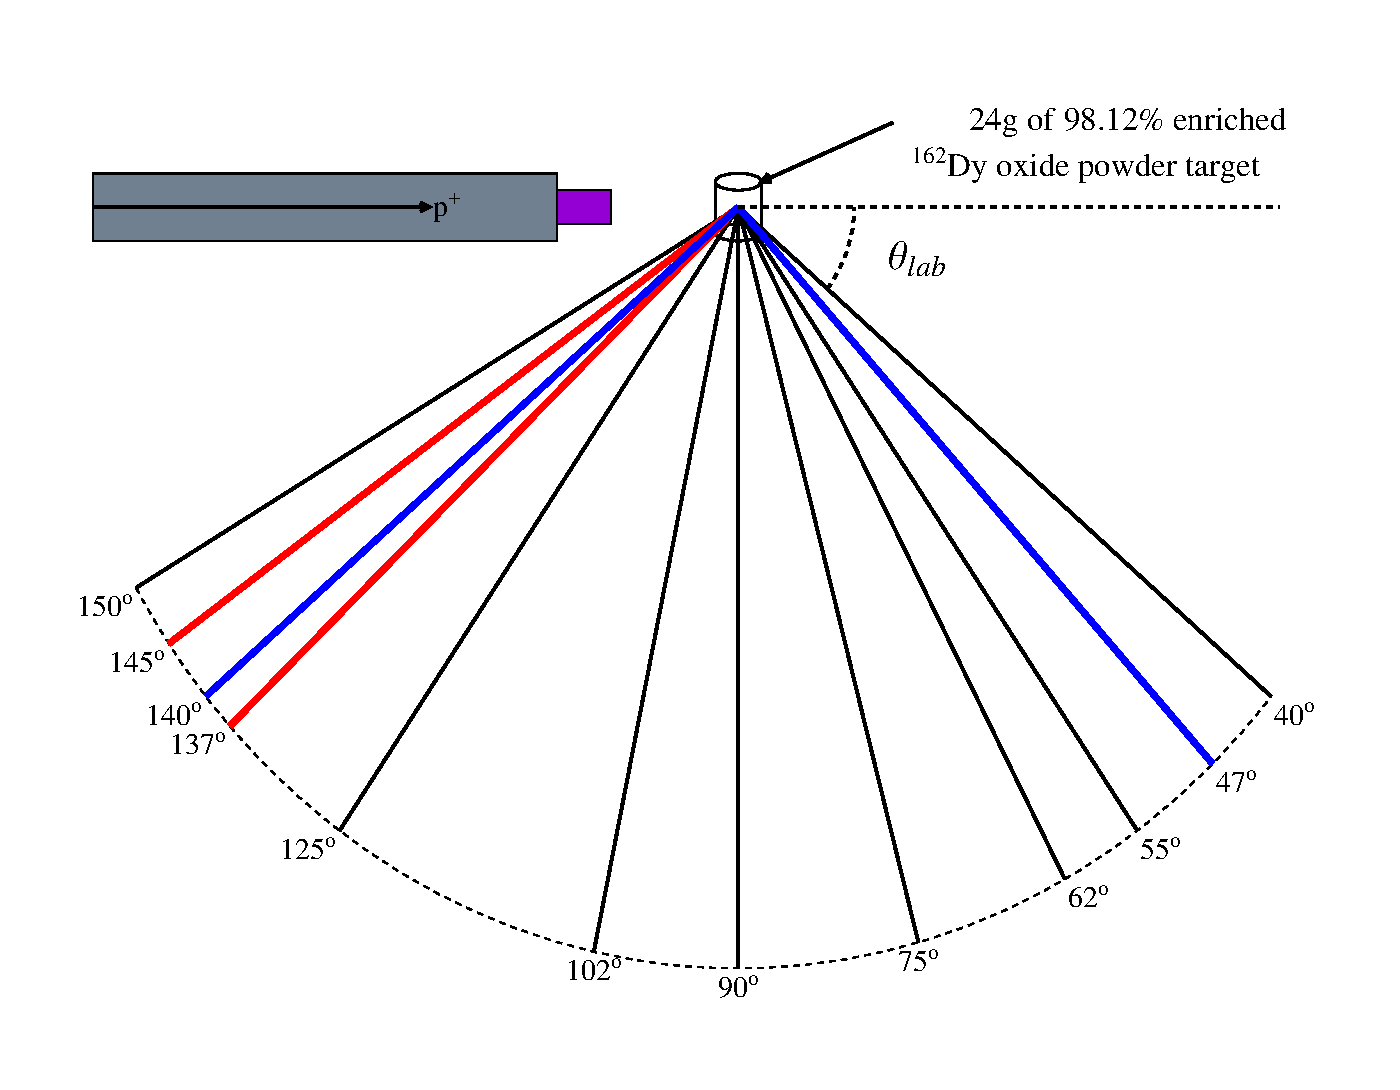
\includegraphics[width=0.95\textwidth]{figures/SciDraw_angular_distributions.eps}
\caption{Angles used in $^{162}$Dy(n,n$^\prime\gamma$) angular distributions. Angles in black are used in all measurements, while angles in red (137$^o$ and 145$^o$) are used for the E$_n$=1.6~MeV measurements and angles in blue are used for both E$_n$=2.2 and 3.1~MeV datasets. \label{fig:SciDraw_angular_distributions}}
\end{figure}

Once data is collected for both experimental campaigns, we carry out the analysis process to extract the various experimental quantities needed for nuclear structure studies (lifetimes of excited states, branching ratios/absolute intensities of $\gamma$-rays, etc) outlined in \S \ref{chp:Analysis}.